\section{TRIỂN KHAI VÀ KIỂM THỬ}

\subsection{Môi trường mô phỏng Mininet}
Đồ án được triển khai trên nền tảng Mininet Network Emulator. Khác với các công cụ như Packet Tracer hay GNS3, Mininet giả lập trực tiếp trên kernel của Linux. Các Switch được sử dụng là Open vSwitch (OVS) và các Router chạy nền tảng định tuyến mã nguồn mở FRRouting (FRR) để giả lập chân thực nhất giao thức OSPF và LDP.

\subsection{Kiểm tra sự hội tụ định tuyến}
Sau khi hệ thống khởi động, quá trình hội tụ định tuyến mất khoảng 30-40 giây. Các bảng định tuyến OSPF và LDP Neighborhood được thiết lập thành công.

\begin{figure}[H]
    \centering
    % [NOTE] CHỤP ẢNH MÀN HÌNH MININET KHI CHẠY LỆNH SHOW IP ROUTE VÀ DÁN VÀO ĐÂY
    % \includegraphics[width=0.8\textwidth]{image/routing_table.png}
    \caption{Bảng định tuyến OSPF hội tụ thành công}
    \label{fig:ospf_route}
\end{figure}
\textit{\textbf{Giải thích minh chứng:} Bảng định tuyến trên cho thấy các router biên (PE) đã học được toàn bộ các đường mạng của khách hàng thông qua OSPF (ký hiệu O). Điều này chứng minh cấu hình IGP đã hoạt động hoàn hảo và không xảy ra vòng lặp định tuyến.}

\subsection{Kiểm tra chuyển mạch nhãn bằng Traceroute}
Để chứng minh hệ thống MPLS đang hoạt động thực sự, công cụ \texttt{traceroute} được sử dụng từ máy hA1 (Site A) đến máy hC1 (Site C).

\begin{figure}[H]
    \centering
    % [NOTE] CHỤP ẢNH MÀN HÌNH MININET KHI CHẠY LỆNH TRACEROUTE VÀ DÁN VÀO ĐÂY
    % 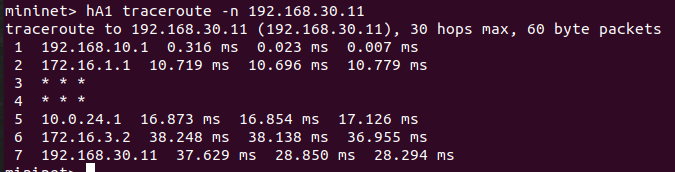
\includegraphics[width=0.8\textwidth]{image/traceroute_mpls.png}
    \caption{Kết quả Traceroute hiển thị nhãn MPLS (Labels)}
    \label{fig:traceroute}
\end{figure}
\textit{\textbf{Giải thích minh chứng:} Kết quả lệnh Traceroute giữa các chi nhánh cho thấy sự xuất hiện của nhãn MPLS tại các trạm trung gian (Provider Routers). Điều này khẳng định gói tin không hề được định tuyến theo IP truyền thống mà đang được "chuyển mạch nhãn" (Label Switching) với tốc độ cao, hoàn thành đúng trọng tâm nghiên cứu của đề tài.}

Như hình trên, tại các hop trung gian qua mạng lõi, gói tin mang theo các nhãn (Labels) chứng tỏ quá trình Label Switching đã diễn ra chính xác theo cơ sở lý thuyết.

\subsection{Đo lường hiệu năng tổng thể}
Việc đo lường hiệu năng được tự động hóa thông qua kịch bản Python, sử dụng lệnh \texttt{ping} (để đo độ trễ) và \texttt{iperf} (để đo thông lượng và Jitter). Kết quả được xuất trực tiếp ra file Excel.

\begin{figure}[H]
    \centering
    % [NOTE] CHỤP ẢNH MÀN HÌNH MININET KHI CHẠY LỆNH THỐNG KÊ HIỆU NĂNG HOẶC ẢNH CHỤP TỪ EXCEL
    % \includegraphics[width=0.9\textwidth]{image/performance_test.png}
    \caption{Báo cáo kết quả đo lường hiệu năng tự động}
    \label{fig:performance_table}
\end{figure}
\textit{\textbf{Giải thích minh chứng:} Bảng kết quả trên (được xuất tự động từ Script Python ra Excel) tổng hợp các thông số hiệu năng cốt lõi như RTT (Độ trễ), Throughput (Băng thông), và Jitter (Độ trễ biến thiên) cho mọi kịch bản giao tiếp giữa 3 kiến trúc LAN (Flat, 3-Tier, Leaf-Spine). Số liệu này là cơ sở dữ liệu thực nghiệm để phân tích ưu nhược điểm ở chương sau.}
